%
%  $Description: Project Final Report for CSE 825$
%
%  $Authors: Vince Fasburg, Bonnie Reiff, Josh Thomas $
%  $Date: 2015/04/13 $
%  $Revision: 1.1 $
%

%\documentclass{ieee}
\documentclass[pagenumbers]{ieee}

%------------------------------------------------------------------------- 
%
% to produce page numbers, bottom centered, in the output. Default is 
% no page numbers for camera-ready copy.
%
%------------------------------------------------------------------------- 

\usepackage{times}
\usepackage{graphicx}

\begin{document}

\title{CSE 825: Project Final Report \\
CAPTCHA-Enabled HID Driver for Prevention of USB Keyboard and Mouse Spoofing\\
}

\author{Vince Fasburg, Bonnie Reiff, and Josh Thomas\\
Dept of Computer Science and Engineering, Michigan State University\\
East Lansing, MI, USA\\
\{Vincent.Fasburg, Bonnie.Reiff, Josh.Thomas\}@ge.com\\
}

\maketitle
\thispagestyle{empty}

%------------------------------------------------------------------------- 
\section{Overview}

Universal Serial Bus (USB) technology has become ubiquitous within our society since the turn of the twenty-first century. This type of the connection has become the standard for computer peripherals such as keyboards, mouses, printers, and external disk drives. USB has also become a common method of connecting devices such as smart phones and digital cameras to computers for power supply and media transfer. It is important for this project to note that all hardware attached to the computer via USB (and other protocols as well) requires an individual device driver in order to enable communication with the computer. Device drivers provide a software interface between the computer and the hardware, allowing the computer to access functions without knowing the exact details of the hardware. Typically, installation of a new device driver is the only obvious notification from a computer desktop that a USB device has been plugged into the computer \textemdash{} the operating system will not ask the user if he or she wishes to allow the device.

This project will focus on the emulation of Human Interface Devices (HIDs), specifically a keyboard and a mouse, through the use of a programmable microcontroller (the Teensy). More will be explained about how this emulation is possible in the ``Approach" section of this report. The future findings of this project can be extended to other USB-connected devices as well, as demonstrated by Karsten Nohl and Jakob Lell at the Black Hat USA Conference in 2014 when they reprogrammed a USB flash memory device to emulate HIDs \cite{nohl}. Through use of keyboard commands and shell scripting, as well as mouse automation to interact with GUI elements, the microcontroller can essentially perform any task available for the current privilege level of the system within seconds, unbeknownst to to user. In order to launch these attacks, the malicious hacker need only plug in the USB device for a short amount of time. For example, this can be done if a user leaves a computer unlocked. Alternatively, the malicious hacker may get the user to plug the device in themselves, as users tend to have a trust that USB devices will not run any programs on their computers without their consent.

%This class of attacks is potentially very dangerous because once the program has the ability to the use the keyboard and mouse, a Linux terminal can be opened to do almost anything to the system, for example, ``rm -rf *'' which would recursively wipes all of the files from the current directory on the drive. The program could easily run without the user being aware since a terminal window could be opened up and immediately minimized while the program is still running. After only a few seconds, the program could be finished running and have the terminal window closed all before the user realizes anything is wrong.

With this background in mind, the proposed project has the goal of answering three questions through both research and implementation:

\begin{enumerate}
\item \textit{What is the extent of attacks the can be performed using USB-HID emulation?}

Initial research for this project has shown attacks on Windows and Apple PC operating systems that include actions such as setting up a reverse shell and changing the Domain Name System (DNS) server (see the ``Previous Work" section for full explanations and citations). The proposed project will explore how these attacks, as well as many others, can be implemented for a  Linux operating system using a programmable USB microcontroller. This suite of attacks will be also be used during the second portion of the project, in which defenses against these attacks will be explored.

\item \textit{What are the existing defenses against HID emulation attacks?}

This question is essentially answered in this project proposal in the ``Previous Work" section, but is included in the Problem Definition because it will be important to final report for the project. The goal of the project is for the team to design defenses against USB-HID emulation attacks, and thus it is important to know this information  in order to compare the approaches that have been taken on features such as feasibility, strength, etc.

\item \textit{Can drivers be designed for USB mouses and keyboards to defend against HID emulation attacks?}

This final question is the most essential and significant to the project as it will require designing and implementing a new concept for USB-HID devices, as well imagining the ways in which the newly implemented defenses can be weakened. The overall goal is to implement drivers for USB mouses and keyboards that have the ability to distinguish between emulated (malicious) devices and human-controlled devices. As will be explained in the following sections, the team has some initial ideas on how this can be done, but there are weaknesses to those ideas that will need to be overcome.

\end{enumerate}

%------------------------------------------------------------------------- 

\section{Previous Work}

The Teensy microcontroller has been used for many purposes, including mounting several different HID based attacks on various systems that accept input from USB human interface devices. An excellent resource that demonstrates the need for HID authentication is the website of Samy Kamkar \cite{samy}, in which the author shows an attack he calls ``USBDriveby''. The USBDriveby attack uses a Teensy microcontroller, emulating a keyboard and a mouse simultaneously,  to create a permanent connection to a remote server that is controlled by the attacker.  This connection will be re-established regularly so that the attacker can issue commands to the machine at any point in the future, including after the microcontroller has been disconnected from the victim's machine.

This example of an emulated HID-based attack serves to show the severity with which a system can be compromised when a malicious USB device is connected for even a short period of time, and without requiring an administrator password. Although the USBDriveby attack was created for the Apple OSX operating system, similar attacks may be possible on any other system that accepts USB input devices. The list of potential attacks is very large, including attacks with various effects to the victim, and ranging from very simple to very complex in implementation.

Although some attempts have been made to develop a mechanism for the authentication of USB devices, much less attention has been paid to the authentication of USB human interface devices. In a paper \cite{wang} proposing an extension to a USB driver to authenticate USB connections, the proposed 2-way authentication mechanism specifically excludes ``non-programmable devices'' such as a USB keyboard. This seems sensible, but leaves a system vulnerable to programmed attacks hiding inside a ``non-programmable device''.

Among the literature dealing with USB device security, some papers such as ``Plug \& Prey: Malicious USB Devices'' \cite{crenshaw} come closer to a solution regarding malicious HIDs. The paper describes how, on Windows, you can use registry changes to prevent USB devices from being installed. However, this would prevent legitimate HIDs from being installed also, unless a whitelist of vendor IDs and product IDs is used to allow certain devices. However, these properties can be spoofed, so the Teensy device may appear to be a whitelisted device.

The final suggestion in this paper is to apply settings to allow administrators to override the policy preventing the installation of a HID. This technique would run into problems if the device in question were the first HID to be connected to the machine, as the user would have no way to allow the installation. Furthermore, it requires administrative privileges to plug in a keyboard or mouse. The mechanism to disable installing USB devices is very different for Linux system, but the results and limitations are roughly the same.

A novel approach to USB authentication specifically for HIDs was proposed by Barbhuiya et al. \cite{barbhuiya}, which relies on either continuous or periodic authentication based on keystroke dynamics, including metrics such as the speed of typing, and the relative times of presses and releases of the keys. This method uses a stored profile of typing behaviors from the authentic user to determine whether the keystroke dynamics exhibited by the inputs are a match to the known patterns. If the keystroke dynamics are determined not to match the stored profile, the input will not be processed.

The keyboard dynamics approach to preventing emulated HID attacks would likely succeed most of the time. However, there are some significant drawbacks in this type of technique from a usability standpoint, stemming from both false positive and false negative authentication. Consider that an attack from a malicious device may be extremely short, and thus more likely to be unintentionally allowed through the authentication (consider the command ``rm -rf *''). If the malicious device were programmed to enter input in a human seeming way (perhaps emulating keyboard dynamics of an average human), there is a significant chance that small amounts of inputs would be accepted \cite{shahzad}. Furthermore, a user using a computer equipped with keystroke dynamics based authentication may reject input from a legitimate user if keystroke patterns change do to any variation in the environment or the user. Lastly, the principles of keyboard dynamics cannot easily be generalized to include authentication for a mouse as well as a keyboard.

Finally, at the 2014 Las Vegas Black Hat Security Conference, Karsten Nohl and Jakob Lell presented several USB based attacks that they collectively referred to as BadUSB \cite{nohl}. Among the attacks described is the malicious emulation of a HID. This section of the presentation describes how an emulated keyboard could be used to steal the administrative password on a Linux system, then allowing the device to perform other actions using the sudo command. The only defenses proposed in this presentation that would be suitable against an emulated keyboard or mouse were to block USB devices entirely, or by using a blacklist or whitelist of device types. As stated previously, such defenses can easily be overcome by spoofing a legitimate device ID.

%------------------------------------------------------------------------- 

\section{Approach}

This project includes two main parts which include first exploiting a few weaknesses in a computer system by creating a suite of attacks, then offering a solution to those weaknesses by developing a method to prevent future attacks. This section will describe the approach for each part of the project.

For the first part of the project, the team programmed a Teensy microcontroller, shown in Figure~\ref{fig:Teensy}, to run a suite of attacks on a Linux operating system. The main idea was to emulate a USB keyboard and mouse with the Teensy so that the computer's Linux operating system would recognize the Teensy as a ``safe" device. This is easily achievable after installing the Arduino and Teensyduino software on the computer being used to program the Teensy using the development environment option to use a board that emulates a USB keyboard and mouse. Once the operating system believes that the Teensy is a safe device, the program can send keyboard or mouse commands to the operating system. The operating system should not notice anything different about these commands as compared to the commands coming from an actual keyboard or mouse. A broad range of attacks were created, including some which would require administrative privileges as described in further detail in Section~\ref{section:teensy}.

\begin{figure}[H]
   \center{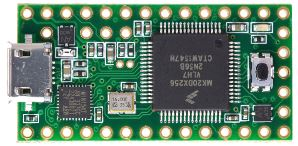
\includegraphics[width=1\linewidth]{Pictures/Teensy}}
   \caption{Teensy Microcontroller}
   \label{fig:Teensy}
\end{figure}

For the second part of the project, the team worked on preventing the attacks that were created in the first part by creating a modification to the Linux driver which handles USB devices such as a keyboard and mouse. The goal of this modification is to authenticate the USB device before any attached keyboard or mouse is allowed to be used normally.

In order to authenticate the USB device, a basic Turing test is used to determine if the input device is being used by a computer or a human. Essentially, a Turing test is a test of a machine's ability to exhibit human behavior indistinguishable of that of a human \cite{turing}. A common way to administer this test is through the use of a random text Captcha. 

The program installed on the Teensy would not know what the random captcha text is going to be, so a human user is required to type in the letters before the keyboard is allowed to be used. In addition, the mouse is verified by requiring the user to hover over the letters of the captcha on a virtual keyboard with the mouse. If the captcha is not entered correctly, the test fails and no other input is allowed from the device until the captcha is completed correctly.

%------------------------------------------------------------------------- 

\section{Threat Model}
The type of attack that is explored in this paper employs a very specific set of capabilities, and is tends to be subject to certain limitations in functionality. Although the Teensy microcontroller was the primary focus in this paper, there are other models of microcontroller capable of emulating HIDs  \cite{captcha}, and some of them have different properties which may warrant separate consideration. 

The most basic version of the attack considered here is the type of attack for which examples are provided in this paper. These attacks involve using preprogrammed actions of a keyboard and/or mouse that run automatically on the Teensy microcontroller when the device is plugged into a host system’s USB port. Although the Teensy microcontroller cannot be programmed to be perceived simultaneously by a host system as both an HID and another type of device such as a flash drive (at least not without significant customization), the proposed solution is meant to be effective against a device that does employ this capability, as long as this solution is run in conjunction an operating system or setting that does not execute programs on newly found devices without user confirmation.

For our purposes, the assumption is made that the malicious device is not capable of emulating a display. Devices that are able to emulate a display as well as an input device may be able to ``view'' the captcha on the emulated screen. It would then be theoretically possible to use an OCR technology to recognize the characters of the captcha and type them into the captcha window, thus defeating the safeguard. Although this possibility is out of scope for current purposes, it is unlikely to be successful due to a number of safeguards already in place. Even if the malicious device were powerful enough to act as a keyboard and a display as well as performing Optical Character Recognition (OCR) functions,  it would still be difficult for an attacker to cause the GUI to appear on the emulated display, because the window is not resizeable or moveable once the input restrictions are in place. Furthermore, if (as a future improvement), the current captcha were replaced with a captcha service where the captchas are specifically designed to defeat OCR, this further reduces the likelihood that any OCR based method to circumvent the proposed solution would be successful.

The type of attack considered here would generally be used when an attacker lacks either physical access or login privileges on the target machine. If an attacker did already have physical and login access, an HID emulation device would do little more than function as a faster method of typing commands than the attacker could do by hand. Instead, this type of attack would be used in combination with social engineering intended to trick a legitimate user of the machine into plugging in the malicious device. For this reason, it is assumed that the attacker cannot access the host machine directly at the time of the attack, in which case the attacker could simply complete the captcha manually.

Finally, the types of attacks that are possible depend greatly on the tools that are installed on the host system. This requires that the attacker be able to predict what operating system is running on the victim machine, and the programs that are installed on it.  In the Teensy code examples used here, only programs that come pre-installed on the 64-bit Ubuntu 14.04 LTS are used. This makes it a very safe assumption that the attacks would be successful on a system running a standard installation of this operating system. 
%------------------------------------------------------------------------- 

\section{Technical Details}

%------------------------------------------------------------------------- 

\subsection{Teensy Attacks}
\label{section:teensy}
\label{section:teensy}
This section describes the code developed to be loaded directly onto the Teensy microcontroller, which performs a variety of malicious actions. The purpose of these attacks is to provide examples of the types of security threats that exist in operating systems that do not require any authentication of USB human interface devices. Each of the following attacks describes an attack and how it was implemented, and suggests ways that the attacks could be improved.

\begin{description}
\item[Delete All Files] \hfill \\
This is the simplest attack, which simply spawns a new terminal window (using the shortcut ctrl+alt+t) and would then enter the command “rm -rf *”. This attack would simply erase the entire hard drive of the victim’s machine. Files deleted in this way may require time consuming or costly measures to be taken to restore the data, if it can be recovered at all. An even more effective version of this command would be to invoke a short script that wrote random data over the entire disk, making it extremely difficult or impossible to recover any overwritten data. In order to test this script, the real command is not used, but instead the line “ALL FILES DELETED” is simply printed to the screen. This is used only for testing and to prevent the accidental deletion of a user’s files. 

\item[Steal Files] \hfill \\
For an attacker who is not satisfied with simply deleting a victim’s files, but would instead prefer to keep them for himself, this attack can be used to transfer any files an attacker wants to a server under the control of the attacker. For this attack, we set up a server, using an inexpensive home router, that can be accessed from anywhere over FTP. The Teensy program uses the built-in ftp tool to transfer any file containing the word “secret” from the victim’s computer to the IP address of this server.  If the attacker did not know exactly what files he would want from the victim, he could easily transfer a large number of files to this server, such as the victim’s entire /home directory. If transferring a potentially large number of files, it may be useful to add commands to the Teensy code to camouflage the fact that the transfers are taking place, as they may take enough time to complete that the user realizes what is happening and cancels the transfer. The transfer could be camouflaged, for example, by minimizing the terminal window performing the transfers or continuously spawning new windows to confuse the user and buy time for the transfer to complete.

\item[Reverse Shell] \hfill \\
A “reverse shell” into a machine is a term used to describe a terminal on a remote computer which connects to a target machine, and is capable of executing commands in the target machine’s environment. An attacker creating a reverse shell on a victim’s machine will be able to execute arbitrary commands from remotely, thus effectively putting the victim machine in complete control of the victim’s machine. 

There are many ways to open a reverse shell on an Ubuntu machine, but this example attack uses a perl script to connect from the victim’s computer directly to an open port on the attacker’s computer, and await commands from the attacker. This technique was chosen because it requires very few keystrokes to initiate the connection, making it possible to execute the command quickly from the Teensy without a user being aware.  The Teensy code for this attack was adapted from a perl script that is freely available on the internet  \cite{pentest}. Since perl is available by default with the Ubuntu 14.04 installation, the attacker can be relatively certain that the attack will work properly on the victim’s machine, assuming that the victim is connected to the internet at the time the malicious Teensy device is inserted. 

The version of this attack provided for this proof-of-concept is very simple, but there are potential enhancements that would allow this principle to be extended to make the attack even more dangerous. For example, the Teensy could easily store the script in the /etc/init.d folder instead of simply executing it in a terminal. The result would be that every time the victim’s system is rebooted, it would attempt to connect to the attacker’s machine, ensuring that the attacker has continuous access to the machine, even after it is rebooted.  Opening the reverse shell in this way also would not show any output, further reducing the probability that an attacker would realize that his system has been compromised. 

\item[Steal Password/Create Account] \hfill \\
This example attack contains two parts. The purpose of the first part of this attack is to obtain the root password. Once the root password is obtained, the Teensy can use this password to perform many commands that require root privileges and cannot be executed without entering a password.  In order to capture the password from the user, this example employs a social engineering tactic to trick the user into providing the root password. The Teensy spawns a terminal and types a message explaining that the user needs to install a driver package to use the new device, and then provides the same prompt for the root user’s password that is normally requested when a command that requires root privileges is attempted (such as installing any new software). If the user is fooled into believing that this is a legitimate message from the operating system, then the user will type the root password into the terminal.

Since the Teensy microcontroller is acting only as a keyboard, it is not capable of accepting the password and storing it for later use. To get around this problem, this example includes the Teensy first typing commands into the terminal which executes a continuous loop, which sleeps until the contents of a temporary file are changed.  After this loop is set up, the screen is quickly cleared before the user has a chance to notice the commands. Once user types in the root password, the password is stored in the temporary file and is read in from the looping execution thread. This loop can now execute the commands that require the root password.

Since the “sudo” command (the command that executes another command as root and requires a password) has an option to allow the password to be provided via the standard in, the password can be piped in from a variable that was set from the value of the temporary file in which the password was stored. This allows the attacker to perform any command he desires, including altering file permission, changing system files, and installing new software.

In this example, once the password has been stolen from the user, the Teensy begins typing commands that add a new root user to the system. Once this is complete, an attacker will be able to log into the system at any time, either over a network or by physically accessing the machine at some later time. Furthermore, this new user has root privileges, so the attacker’s credentials can be used to access or modify any files on the entire system, including those of other users. 

In this version of Linux, the login screen shows all of the different users. Although a system that has many legitimate users may go a long time before the attacker’s login information is noticed, this example takes one more measure to prevent this extra account from being noticed. Before setting up a new account, the Teensy adds a system file that disables the guest account that is enabled by default on Ubuntu 14.04. This guest account is shown as “Guest Session” on the login screen. The new user that is added by the Teensy is called “Guest”, in the hopes that the switch from “Guest Session” to “Guest” would not be readily noticed or seem suspicious to a legitimate user. Suspicion would probably arise, however, if someone attempted to use the Guest account and discovered it required a password.

\item[Mouse] \hfill \\
All of the attacks thus far presented have used only the keyboard to cause malicious behavior. This final example is used to defend the necessity of protecting a newly inserted USB mouse with a captcha as well as a keyboard. Note that the program described in this paper utilizes a restriction of the keyboard to only letters and numbers, and prevents the mouse from clicking.  If only the keyboard were restricted, then a Teensy device posing as both a keyboard and mouse would be able to use the mouse to open a new terminal, as shown in this example. Once this terminal is opened, the Teensy could type and command that consists of only letters and numbers into the terminal without ever completing the captcha.
\end{description}
%------------------------------------------------------------------------- 

\subsection{Java GUI}
\label{section:gui}
In order for the user to validate the USB device, a Graphical User Interface (GUI) was created with a captcha and a method to validate both with the mouse and the keyboard. The GUI was created in Java with the basic components of the Java Swing \cite{kim} library as shown in Figure~\ref{fig:JavaGUI}.

\begin{figure}[H]
	\center{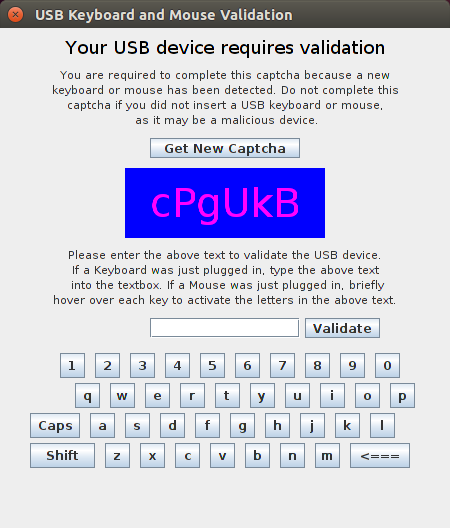
\includegraphics[width=1\linewidth]{Pictures/JavaGUI}}
	\caption{GUI to Validate USB Device}
	\label{fig:JavaGUI}
\end{figure}

The captcha was generated with a random sequence of six alphanumeric characters in both upper and lower case. The current captcha is non-web based and is generated completely with the use of a java class. The user can generate a new captcha with the ``Get New Captcha'' button in the event one of the captchas is unreadable. The background color, foreground color, and font also have the ability to be randomized with a blacklist in place to prevent certain color combinations.

The GUI has been designed to always stay on top of other windows as well as always remain in focus. This prevents a malicious program from trying to open a terminal or closing out of the GUI. In addition, each time the GUI opens, it appears in a randomized location on the screen. This location is bounded to prevent the GUI from opening up partially or fully off of the screen. This prevents an emulation program from pre-programming where the buttons on the GUI will be located then using this information to try to close it or read the captcha with some kind of computer vision. The ``x'' to close the GUI has also been disabled so the GUI can only be closed with the correct input of the captcha.

There are two methods to input the captcha text for validation. The first method would be used if a keyboard needed to be validated. The user would simply type the captcha text directly into the blank textbox and then press enter or briefly hover over the ``Validate'' button.

The second method would be used if a mouse needed to be validated. The user would use the virtual keyboard on the GUI to type the captcha into the textbox. As another security feature, clicking of the mouse has been disabled. The user would activate the keys by briefly hovering \cite{hover} over each key that is needed. When finished, the user can also briefly hover over the ``Validate'' button.

If the captcha is incorrect, an error message would appear along with a new captcha to attempt. With a correct captcha, the GUI is closed and the user gains full access of both the keyboard and mouse.

%------------------------------------------------------------------------- 

\subsection{Kernel}

The driver modification development for this paper was done on a computer running Ubuntu 14.04 LTS with a 3.13.0-32 kernel release. The final testing of the new driver occurred using the 3.13.0-46 kernel release due to a software update. The baseline code used for the driver modification work was the latest stable kernel found on The Linux Kernel Archives website \cite{kernel}, version 3.19.3. 

The work for the driver modification was focused entirely within the \texttt{linux-3.19/drivers/hid/usbhid} subdirectory and made use of the header files at \texttt{linux-3.19/include/linux}. The appropriate drivers for the project were discovered by browsing the various subfolders of the ``drivers'' directory of the linux source code and by subsquently using Linux system logging functionality while connecting and disconnecting a USB-HID device to test that the appropriate drivers were found (see the section below on the \texttt{call\_usermodehelper} function for more detail). Through this process, the ``usbhid", ``usbmouse", and ``usbkbd" drivers were discovered. For the scope of this project, only the usbhid driver needed to be modified, but the code for the usbmouse and usbkbd drivers is important to understand for possible future improvements to this defense against USB-HID emulation attacks.

\subsubsection{Initial Driver Compilation}

In order to get the driver source code in the \texttt{drivers/hid/usbhid} directory to compile initially after download, several modifications had to be made to the provided Makefile, which uses the ``kbuild'' Linux kernel build system. First, Makefile targets ``all'' and ``clean'' (using the syntax for building an external module) were added. The ``all'' target is set to \texttt{make -C lib/modules/\$(KVERSION)/build M=\$(PWD) modules}, where \texttt{KVERSION = \$(shell uname -r)}. Similarly, the ``clean'' target is set to \texttt{make -C /lib/modules/\$(KVERSION)/build M=\$(PWD) clean}. The ``\texttt{-C}'' option in both of these targets indicates that the path to the kernel source is being provided \textemdash \ the \texttt{make} program changes to this directory during the build process and then changes back to the local directory when the process is complete. The \texttt{KVERSION} variable expands to the current kernel release. For example, if \texttt{KVERSION = 3.13.0-46-generic}, the kernel version is 3.13.0 and ``46'' refers to the release number determined by the patches applied during software updates. The ``\texttt{M=<directory>}'' option is what indicates that an external module is being built and provides the absolute path to the module. Thus, this Makefile needs to be in the same directory as the usbhid driver code %\cite{kbuild}.

During project development, it was noted that there is a consequence to using the \texttt{uname} program in the Makefile to determine the current kernel release \textemdash \ loadable kernel modules compiled under a specific kernel release can only be installed on that release. Therefore, when the kernel is patched and a new release is created, the driver must be recompiled if the user wishes to include the modified driver in the newest kernel release.

After adding the targets, for any files in the directory that were still producing errors due to unrecognized information from the linux header files when the \texttt{make} program was executed, the appropriate code was copied and pasted locally to eliminate compilation errors.

\subsubsection{\texttt{call\_usermodehelper} Function}

Many common C header files do not exist in the kernel development environment and cannot be included in the kernel programs. Thus, the \texttt{call\_usermodehelper} function was essential to the driver modification work. This function allows user space applications to be invoked from the kernel. The \texttt{call\_usermodehelper} functions combines the functionalities of the \texttt{call\_usermodehelper\_setup} and the \texttt{call\_usermodehelper\_exec} functions, which are both part of the \texttt{usermode-helper} API. The \texttt{call\_usermodehelper\_setup} function prepares a handler for the user space call, whereas the \texttt{call\_usermodehelper\_exec} function invokes the user space call. The \texttt{call\_usermodehelper} function is defined in \texttt{linux-3.19/include/linux/kmod.h} and has four input parameters \cite{ibm}:
\begin{itemize}
\item \textit{char *path}, the path to the program to be executed
\item \textit{char **argv}, the null terminated list of program arguments, including the name of the program at zeroth index
\item \textit{char **envp}, the null terminated list containing environment information 
\item \textit{int wait}, \texttt{UMH\_WAIT\_EXEC} to wait for the user space application to be invoked before continuing, \texttt{UMH\_WAIT\_PROC} to wait for the entire process (including the application running in user space) to complete, or \texttt{UMH\_NO\_WAIT} to include no wait time
\end{itemize}

The newly implemented usage of this function in the usbhid driver is shown in Figure~\ref{fig:usermodehelper_code}.

\begin{figure}[H]
   \center{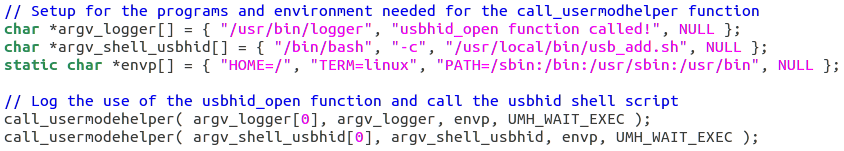
\includegraphics[width=1\linewidth]{Pictures/usermodehelper_code}}
   \caption{\texttt{call\_usermodehelper} additions to the \texttt{usbhid\_open} function}
   \label{fig:usermodehelper_code}
\end{figure}

The appropriate function to modify was then determined using the system log (found at \texttt{/var/log/syslog}). The text logged by the unmodified driver(s) upon insertion and removal of a USB-HID device was searched within the \texttt{drivers} directory of the source to determine a subset of files and functions to test that pertained to the connection and disconnection of the device. System logging calls were then added to this set of functions to choose the exact driver modification location \textemdash \ the \texttt{usbhid\_open} function in hid-core.c, located in the \texttt{drivers/hid/usbhid} directory.

First, only the \texttt{argv\_logger} and \texttt{envp} variables shown above in Figure~\ref{fig:usermodehelper_code} were added, along with the call to the function. The \texttt{envp} is a null terminated array that defines the execution environment for the user space application. The \texttt{argv\_logger} array indicates that the system logger program should be called with one argument \textemdash \ the text to write to the log file. The result of this when any USB-HID device is plugged into the computer is the ``logger'' line displayed in  Figure~\ref{fig:syslog}. Note that the call to \texttt{call\_usermodehelper} uses a wait time of \texttt{UMH\_WAIT\_EXEC}, meaning that the code blocks until the program is executed and then continues.

\begin{figure}[H]
   \center{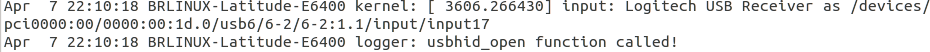
\includegraphics[width=1\linewidth]{Pictures/syslog}}
   \caption{System log showing the \texttt{usbhid\_open} function call}
   \label{fig:syslog}
\end{figure}

Later, after the bash script (to be described in a later section of the paper) was developed, the \texttt{argv\_shell\_usbhid} array and call to the bash program were added. The bash program is passed two arguments, ``\texttt{-c}'' and the path to the shell script. The \texttt{-c} option indicates that the shell script should be treated as an executable command, rather than a positional parameter to a command. The previously used call to the system logged was kept to ensure that the \texttt{usbhid\_open} function was being called appropriately in the case that the bash script did not execute correctly. 

\subsubsection{Installation of Modules}

When the kernel source files are compiled in local user space, they produce both regular C object files (.o) and loadable kernel module files (.ko). The following steps then need to be taken to install the new versions of the modules. These steps were scripted as part of the project in order to allow for faster installation and test of changes:

\begin{enumerate}
\item Uninstall the old version of the module at \texttt{/lib/modules/\$(uname -r)/kernel/ drivers/hid/usbhid} using the \texttt{sudo rmmod usbhid.ko} command
\item Copy the new module from local user space to \texttt{/lib/modules/\$(uname -r)/kernel/ drivers/hid/usbhid}
\item Insert the new module using the \texttt{sudo insmod usbhid.ko} command
\end{enumerate} 

To verify the insertion or removal of a module, the \texttt{lsmod} command can be used to show the status of the modules in the Linux kernel. This program also shows the size of each module (which is helpful for distinguishing between different versions), as well as what other modules are dependent on it.

%------------------------------------------------------------------------- 

\subsection{Bash Script}
The script that is called from driver code is responsible for opening the captcha program and for restricting the user input from the keyboard and mouse to ensure that the captcha is completed before any other input can be taken from these HIDs.  The script works by using the modifying the X11 keyboard and mouse mappings using the xmodmap function. Through this function, all keyboard inputs except for letters, numbers, and the shift and enter keys are unmapped (meaning that they will not be received by the operating system or any application) using a pre-defined restricted keyboard map file. All mouse keys are similarly unmapped, disabling all button clicks on any mice connected to the system. 


Once the input restrictions are in place, the script spawns the java jar that opens the captcha completion window. The keyboard and mouse restrictions prevent the user from closing the captcha GUI or performing any other action until the captcha is completed. As a backup to this system, the GUI itself is also programmed to always keep in focus and stay on top of other windows.

The bash script blocks when the captcha GUI is spawned, and waits for the GUI to close. The only way to close the captcha GUI is to complete the captcha, at which point the script will continue. The previous remappings of the keyboard and mouse are then returned to normal, allowing the user to use the keyboard and mouse freely.

In order to make these commands effective on the current user, while running a script from kernel space, several additional steps are needed. Permissions must be explicitly given for the local user to access the X server, and the DISPLAY variable must be exported to give display access to the script.  Every command in the script that interacts with an I/O device needs to be be executed through the local user using the “sudo -u” command. 

These setup steps are also needed if the script is to be run from a udev rule, which can be used to execute a script whenever a certain category of USB device is inserted. This was the original method by which the script was invoked, until it was proven to be feasible to run the script directly from the USB driver within the kernel.

%------------------------------------------------------------------------- 

\section{Experimental Results}

After development of the modified driver was complete and installed on an Ubuntu system, the modified driver was tested against three types of devices: 

\begin{itemize}
\item \textit{USB Flash Drive.}

This test was executed to ensure that the captcha program only appears for human interface devices as opposed to for all USB devices. The computer responded as expected \textemdash \ a File window showing the contents of the USB flash drive was opened and the captcha program did not run. A review of the system log shows that different calls are made for USB file storage devices versus the calls made for USB-HID devices.

\item \textit{USB Mouse and USB Keyboard.}

These tests were executed to ensure that the captcha program runs as expected for the devices on which this research focused. When either of the devices is plugged into a USB port, the captcha program appears. Note that due to the design of the shell script, if the captcha program is active when an additional USB-HID device is connected, the code to restrict the keyboard and mouse functionalities and launch the captcha program is skipped. During the time that the captcha program is active, the user is unable to click with the mouse or use special, non-alphanumeric, keys on the keyboard. As an extra precaution, the captcha program also holds focus to ensure that the user cannot start or interact with any other programs on the computer. When the captcha is successfully completed, the program exits and normal mouse and keyboard functionality are restored. More details on the results of these tests, as well as how users responded to the captcha program, can be found in the following section (``Usability Testing").

\item \textit{Teensy Programmable Microcontroller with attack loaded.}

A Teensy (version 3.1) was set to simultaneously emulate a keyboard, mouse, and joystick (all USB-HID devices) and loaded with each of the attacks described above in the ``Teensy Attacks'' section of the paper. The Teensy was subsequently plugged into a USB port and the system was observed to see what (if anything) occurred before the captcha program loaded. 

The four keyboard-based attacks, in which the Teensy program attempts to open a terminal using the special key sequence CTRL-ALT-T and subsequently execute various malicious commands, were all prevented. Testing revealed that the programs had the ability to open a terminal window, but the captcha program always loaded and grabbed focus before the malicious commands could be performed.

The mouse-based attack, in which the Teensy program opens a terminal without the special character sequence by navigating to the ``Search'' program on the taskbar and searching for the terminal application, also proved to be ineffective against the captcha-enabled driver...

\textbf{TODO (Bonnie, after the Teensy programs have been modified)}

\end{itemize}

%------------------------------------------------------------------------- 

\section{Usability Testing}
Usability testing is used in products that have a user-centered interaction in order to evaluate it by testing on outside users. As a part of the overall testing of the USB verification software, we had individuals who were not part of the development team use the software to see their overall impression of the design. The following summarizes  the outcomes of the study:
\begin{enumerate}
\item Users did not completely understand the idea behind hovering over the buttons to activate them. We found that some users would try to click, and then ended up hovering too long which allowed multiple letters to appear. In future versions of the Java GUI, we could reevaluate the usefulness of the hovering feature. Since the GUI does also keep its own focus and stays on top of other windows, disabling the clicking may not be required. 
\item A few individuals mentioned that the letters on the keyboard were a bit too small. If someone had bad eyesight, it would be even more difficult to see. The size of the text for the buttons should be enlarged so that it is easier to read. In addition, by enlarging the text on the keys, the keys would become larger as well. This could help users ``type" on the keyboard more easily by providing bigger targets to which the mouse can be guided.
\item Lastly, there were comments made on the length of the directions on the page. Most people probably do not want to take the time to read all the through them and may begin completing the captcha before having finished reading. This could lead to the captcha being completed incorrectly or using the wrong method (mouse verification versus keyboard verification). If there is some way to summarize the directions and increase the size of the font to make the user more aware of what to do, that would be very helpful.
\end{enumerate}
%------------------------------------------------------------------------- 

\section{Technical Weaknesses}
\label{section:weakness}
This implementation of the keyboard and mouse restriction contains a vulnerability that allows a short window of time in which commands from the Teensy device were executed before the keyboard and mouse restrictions were imposed. In our testing, there was considerable variability in the number of keystrokes that could be executed by the Teensy before having the input restrictions imposed and the captcha GUI opened. In the best case, there was only enough time to spawn a terminal, and the captcha window appeared before any commands could be issued by the Teensy. However, on the computer that took the most time to open the captcha window, enough keystrokes were allowed through for the Teensy to invoke a short attack, such as “rm -rf *”.  This weakness is a limitation only of the particular implementation, and could be remedied with further work. See Section~\ref{section:Conclusion \& Future Work} for a description of this improvement.

The threat model that was considered in this paper is concerned primarily with the unmodified Teensy microcontroller and similar HID emulation devices. However, it is possible to modify the Teensy microcontroller to connect it to a real keyboard, which will pass keystrokes through a real keyboard.   \cite{pjrc} This makes it possible for an attacker to provide a keyboard with an embedded malicious device to a legitimate user. When the user plugs in the keyboard, the Teensy could wait for the user to complete the captcha (passing through the user’s input as entered on the actual keyboard) and then execute a malicious script once the captcha has been completed. The solution described in this paper would not prevent an attack of this type.

A further limitation of the current implementation is that the user is not limited to completing the captcha using the device that was just plugged in.  Once the captcha window is opened, any keyboard or mouse can be used to complete the captcha. This limitation will only cause the captcha to fail under certain circumstances. For example, assuming that a user understands that the captcha window will only appear when a USB keyboard or mouse is inserted, then the user would not complete the captcha when they thought the device that they inserted was a flash drive. Although the GUI in the captcha window contains a warning to users not to complete the captcha if they did not insert a USB keyboard or mouse, users may still fail to heed this warning, resulting in a successful attack from the malicious device. This limitation can also be eliminated by implementing this protection as described in Section~\ref{section:Conclusion \& Future Work}.

Finally, this implementation is not effective against a USB device that was plugged in when the computer was shut down or sleeping, and was subsequently booted up.  In this case, the bash script is executed, but the captcha GUI is not shown. This fact was discovered in testing and the cause has not been determined. However, a likely cause is that the kernel driver code may execute on boot up before the user environment is set up to the point of being able to run some of the commands in the bash script, such as the interactions with X or the Java installation. If this interpretation of this failure is correct, then the enhancement described in Section~\ref{section:Conclusion \& Future Work} would be expected to fix this problem also.

%------------------------------------------------------------------------- 

\section{Conclusion \& Future Work}

In this paper, we examined the following three aspects of USB-HID emulation attacks on an Ubuntu operating system:

\begin{itemize}
\item The extent of attacks the can be performed using USB-HID emulation with a programmable microcontroller
\item The existing defenses against USB-HID emulation attacks
\item New possibilities for USB-HID driver design to defend against HID emulation attacks
\end{itemize}

The resulting research produced Ubuntu attacks written for the Teensy USB-based microcontroller development system, as well as a modification to the ``usbhid'' Linux driver that has been proven to render malicious Teensy-based attacks ineffective, while still allowing normal use of USB input devices, such as the mouse and keyboard. The driver modification in its current state runs a bash shell script to restrict keyboard and mouse functionality until a team developed captcha GUI (written in Java) is completed successfully.

As this was a proof of concept, in addition to fixing the technical weaknesses explained Section~\ref{section:weakness}, there are several improvements that can be made in future versions of the driver modification. Once such improvement would be to use a more advanced captcha. As stated in Section~\ref{section:gui}, the current captcha is a non-web based random sequence of six alphanumeric characters with randomized background color, foreground color, and font. A more advanced captcha contains characteristics such as letter distortion and strokes through the text, and makes tasks such as segmentation (the ability to spearate one letter from another) difficult, especially without understanding the context of the words \cite{captcha}.

The other two suggested improvements for future work revolve around the concept of containing all elements of the USB-HID validation to ``kernel space'', from where the shell script is initially called. Kernel space is a privileged area of virtual memory reserved for the operating system and most device drivers, whereas user space allows application software to run. Even though the shell script described in the ``Bash Script'' section of this paper is called from device driver code (kernel space), the shell script actually executes in user space, which is not preferable. In order to contain all shell script functionality within kernel space, the restriction of keyboard and mouse functions and the execution of the captcha program would both need to be converted to C code. 

Since interpreted code cannot be run in kernel space, the captcha program would need to be ported to a language other than Java or Python (which are both common computer languages for handling graphics) in order to call the program from the C code \textemdash \ the program would most likely still be called using the \texttt{call\_usermodehelper} function described in the ``Kernel'' section of this paper. In regards to the restriction of keyboard and mouse functions, structures exist in the code for the ``usbmouse'' and ``usbkbd'' drivers (unmodified in the scope of work for this project) that can be modified in a similar manner to how the functionality of these two devices was modified in the shell script. For the available keys on the keyboard, the ``Xmodmap\_orig'' mapping file is  analogous to the \texttt{usb\_kbd\_keycode} array of 256 \texttt{char} types (found in usbkbd.c). There are two ways in which the kernel can restrict the use of special characters on the keyboard. The first option is to edit the \texttt{use\_kbd\_keycode} array to match the ``Xmodmap\_restricted'' file (if the array declaration is made non-constant). The other option is to use the \texttt{input\_report\_key} function, which is called in both the usbmouse and usbkbd interrupt request (``irq'') functions. This function takes in a device, a keycode, and a value (generally with a mask) and reports back the state of the key to the system %\cite{input}
. In order to restrict the use of special characters, the driver can be modified to use this function to ensure that when a special character is typed on the keyboard, the signal is not reported to the system. The ability to use various mouse buttons must be restricted in a similar manner as the mouse buttons are defined in a header file and thus, the available buttons cannot be modified dynamically.

After these improvements to the driver have been developed and tested and input from the usability tests has been incorporated into the captcha-enabled USB-HID driver, the last challenge to face is installation. In the proof of concept version developed for this paper, the bash script must be configured for the current user. Once a solution is developed to either install this script for every user of the system or to dynamically configure the script based on the current user, deployment would simply consist of including the necessary files and updated driver code in the next kernel release.

%------------------------------------------------------------------------- 

\appendix 

%\newpage% -- remove this comment if we want the Appendix and References on a new page

\section{Appendix: Team Contributions}

The major project deliverables and testing of the end product were divided as follows among the team members:

\begin{center}
	\begin{tabular}{ | c | c | }
		\hline \textbf{Project Contribution} & \textbf{Assigned Team Member} \\ \hline
		Teensy code attacks & Vince Fasburg \\ \hline
		Captcha GUI & Josh Thomas \\ \hline
		Driver modification & Bonnie Reiff \\ \hline
		Shell script & Vince Fasburg \\ \hline
		Udev rule research & Vince Fasburg \\ \hline
		Final product testing against attacks & Bonnie Reiff \\ \hline
		Usability testing & Josh Thomas \\ \hline
	\end{tabular}
\end{center}

Each student on the team wrote about his or her own project responsibilities in the final project paper. In addition, the extra paper sections were assigned as follows:

\begin{center}
	\begin{tabular}{ | c | c | }
		\hline \textbf{Team Member} & \textbf{Extra Paper Sections} \\ \hline
		Vince Fasburg & Threat Model, Technical Weaknesses \\ \hline
		Bonnie Reiff &  Future Work \\ \hline
		Josh Thomas & Overview, Previous Work, Approach  \\ \hline
	\end{tabular}
\end{center}

 All team members were responsible for final read through and editing of the final paper.

%------------------------------------------------------------------------- 

\bibliographystyle{ieee}
\bibliography{bibfile}

\end{document}

